\chapter{Literature Review}
Recently, various approaches have been proposed and implemented for intelligent driver assistance system (IDAS). These approaches used classical machine learning methods for object detection which were slow to use in real-time application. Lots of them were developed in case of daytime driving, while others supported night-time driving. However, research of driving in night-time environment is not mature. It is still a hot topic for researchers around the world. There have been many vision-based approaches that try to detect efficiently on-road abnormal moving vehicles. These approaches can be separated into two groups based on the position of cameras: fixed cameras (surveillance) and moving cameras that are mounted on the host moving vehicles. 
\section{Related Works}
The proposed methods in market and academic literature can be grouped by the nature of object detection methods, classification techniques and position of camera(moving or fixed).

Sang Hai-feng et al \cite{hai-feng_hui_dan-yang_2012} proposed a system for video based traffic surveillance system. Their system is composed of three modules: the vehicle detection module, the vehicle tracking module and abnormal behavior identification module. The following figure 2.1 shows their proposed system. In their proposed method 

\begin{figure}[h]
    \centering
    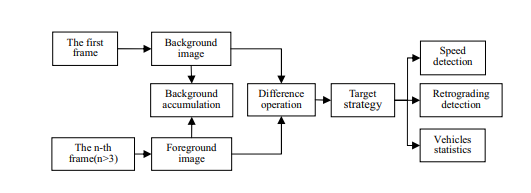
\includegraphics[scale=0.7]{pic_1.png}
    \caption{Proposed system in \cite{hai-feng_hui_dan-yang_2012} }
    \label{fig:my_label}
\end{figure}

\begin{itemize}
    \item Vehicles are detected using background acquisition and vehicle extraction. Background acquisition is used for construction background. The basic idea is that the iterative accumulation of all frames is used as background. Vehicle extraction is done using background subtraction method. Moving targets are detected by the difference between foreground image and background image.
    
    \item Vehicle tracking is done by extracting features of vehicles like  color, edge, block feature, optical flow, perimeter, area, center, corner points and then feature matching is used for tracking of vehicles.
    
    \item Abnormal behaviour detection is done using speed of vehicles. If speed of a vehicle exceeds a particular threshold then it is classified as abnormal.  
\end{itemize}

Lili Cui et al \cite{cui_lili_kehuang} proposed a method for abnormal event detection in traffic video. Their proposed method is based on local features. The researchers proposed a new framework with multiple classifiers which can be trained at the same time but focus on different features. In their work, abnormal events are ranked rather than alarmed with no more information. It is most parts of the framework work in parallel that reduces mistakes passed on. 

The following figure 2.2 shows their proposed framework.

\begin{figure}[h]
    \centering
    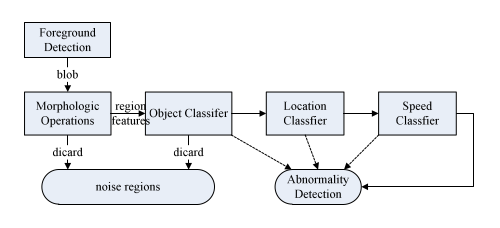
\includegraphics[scale=0.7]{pic_2.png}
    \caption{Proposed system in \cite{cui_lili_kehuang}}
    \label{fig:my_label}
\end{figure}

According to their proposed method
\begin{itemize}
    \item Firstly features are extracted from video frames. For this foreground detection, object velocities are identified. Foreground detection is done using Sigma-Delta filter followed by morphological operators. Object velocities are identified using Lucas-Kanade optical flow analysis algorithm.
    
    \item Abnormal event classification is done with help of local velocity distribution. If a vehicle illegally stops, moves in wrong direction, or exceeds the speed limit, etc., it will have a velocity out of the local range and thus can be classified as abnormal.
\end{itemize}
Cuong Nguyen Khac et al \cite{khac_park_jung_2016} proposed a method for abnormal event detection method and it is a moving camera approach. The following figure shows their proposed method 

\begin{figure}[h]
    \centering
    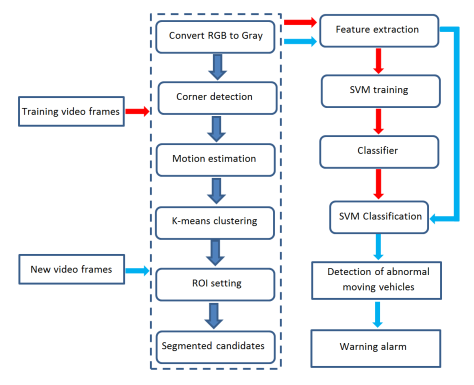
\includegraphics[scale=0.7]{pic_3.png}
    \caption{Proposed method in \cite{khac_park_jung_2016}}
    \label{fig:my_label}
\end{figure}

According to their method 
\begin{itemize}
    \item Firstly, each RGB frames from real time video is converted to gray-scale images to facilitate corner extraction step. Shi-Tomasi corner detector is used to obtain a sparse distribution of corner points.
    
    \item The set of extracted corner points from a couple of frames are used to determine their optical flows using pyramidal Lucas-Kanade optical flow algorithm. The estimated set of optical flows can be used to describe the motion of all moving objects along the time domain.
    
    \item Based on the observation, a practical threshold range is used to eliminate the set of short vectors(very similar to host vehicle) that belong to the safety moving vehicle with respect to the host moving vehicle.
    
    \item The remaining motion vectors are clustered into K clusters by using K-means clustering algorithm. K-means algorithm returns the specific two dimensional coordinates of the centers and the vectors of each group. These K groups are considered as K vehicle candidates.
    
    \item Out these K vehicle candidates abnormal vehicle detection is done using a SVM classifier. This SVM classifier is initially trained using 1000 frames from real life traffic videos and features used are HOG (Histogram of Oriented Gradients) and LBP (Local Binary Pattern) [16].HOG feature focuses to describe shape information while LBP emphasizes texture information.
\end{itemize}

Their method gives accuracy of 91.96\%.